\chapter{背景知識}

\section{NAND FLASH Memory}\label{s2.1}
\indent
是電子抹除式可程式化唯讀記憶體(Electrically-Erasable Programmable Read-Only Memory,簡稱EEPROM或E2PROM)的其中一種,通常為 SSD、記憶卡、以及隨身碟的主要材料元件,可透過電子方式多次複寫,而這種元件具有以下特性:\\
$\bullet$ Erase before write \\
$\bullet$ Limited P/E cycles \\
$\bullet$ Asymmertic Program/Erase unit \\
以下將一一介紹這些特性。

\subsection{Wear}\label{s2.1.1}
\indent
又稱 Program/Erase Cycle,簡稱P/E cycle。重複的寫入會為用來儲存電子的 Flash Memory Cell 帶來不可逆的損害,而隨著 Flash Memory 的製造商想要把越多的位元塞進一個 Cell 裡面,這些 Cell 的壽命就越來越少,例如 MLC,TLC,QLC 等等。
\begin{figure}[H]
    \centering
    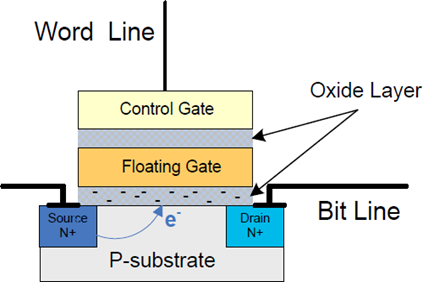
\includegraphics[width=0.35\textwidth]{picture/ch2/wear.png}
    \caption{暫定:Flash Memory Cell 示意圖}
    \label{f2.1}
\end{figure}

\subsection{Retention loss}\label{s2.1.2}
\indent
存在 Flash Memory Cell 中的電子可能會隨著時間增加而外洩,增加 SSD 正確讀取資料的困難度。這個問題可以藉由抹除資料後來重置狀態,但是重置會消耗寫入次數。
\begin{figure}[H]
    \centering
    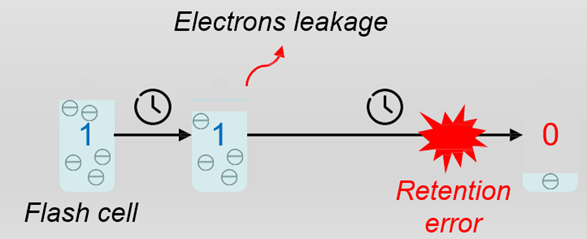
\includegraphics[width=0.5\textwidth]{picture/ch2/retention_loss.png}
    \caption{暫定:Retention loss 示意圖}
    \label{f2.2}
\end{figure}

\subsection{Disturbance}\label{s2.1.3}
\indent
從一個 WordLine 讀取或寫入資料可能會造成電子外洩至旁邊的 WordLine,也就說,只要讀取資料就有機會影響所選 WordLine 鄰居。
\begin{figure}[H]
    \centering
    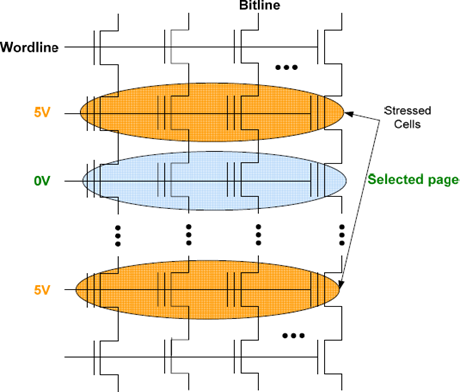
\includegraphics[width=0.5\textwidth]{picture/ch2/disturbance.png}
    \caption{暫定:Disturbance 示意圖}
    \label{f2.3}
\end{figure}

\section{SSD}\label{s2.2}
\indent
SSD,全名:Solid State Drive,中文:固態硬碟,裡面的主要儲存元件為上述提到的 Flash Memory,而為了降低上述所提到問題造成資料錯誤,SSD的製造商通常都會將 FTL 導入至 SSD 裡面。

\subsection{FTL}\label{s2.2.1}
\indent
全名:Flash Translation Layer,簡稱 FTL,負責管理所有為了降低 Flash Memory 帶來的錯誤而產生的技術,再模擬成一個普通的硬碟,讓作業系統管理SSD與其他硬碟的方式一致。而其中的技術通常包含:\\
$\bullet$ Mapping Table \\
$\bullet$ Garbage Collection \\
$\bullet$ Wear Leveling \\
以下將一一介紹這些技術。

\subsection{Wear Leveling}\label{s2.2.2}
\indent
因為上述的問題,如果每次都寫入同一個位置會導致 Cell 的壽命會銳減,因此為了延長每個 Cell的壽命,寫入時需要從壽命比較長的開始寫入,以平衡整體 SSD 的壽命。所以 SSD 會記錄每個 Cell 的存取次數,來決定下次要寫入到哪裡。
而這項技術會與 Mapping Table 結合,

\subsection{Mapping Table}\label{s2.2.3}
\indent
為了實作 Wear Leveling,又要讓 Host 覺得跟傳統硬碟的管理方式一致,因此在 SSD 中就多了一個轉換表,紀錄 Host 傳給SSD的 Logical Block Address 是對應到實際的哪個Physical Address,通常是存成一個 Table,來維護這個功能。

\subsection{Garbage Collection}\label{s2.2.4}
\indent
因為清除資料時的延遲較高,也因為 Disturbance 而要每過一段時間就將還有效的資料讀取出來寫入至新的區域裡面。
Garbage Collection 就是紀錄哪些區域要清除資料,或是挑選哪些資料要讀取出來再放到新的區域。
並在 SSD 控制器較為閒置時再執行。

\section{Open Channle SSD}\label{s2.3}
\indent
雖然 SSD 已經有了上述技術來管理以及延長壽命,不過由於這些技術仰賴於 SSD 內部的控制器及韌體管理,Host 完全不知情,所以寫入及讀取的延遲時間取決於韌體以及SSD控制器的穩定度,而為了讓延遲時間能夠掌控在 Host 的手上,也同時為了降低成本,於是有了Open Channel SSD。Open Channle SSD 將下列技術往上交給 Host 管理。\\
$\bullet$ Mapping Table \\
$\bullet$ Garbage Collection \\
$\bullet$ 部分的 Wear Leveling

\section{LightNVM}\label{s2.4}
\indent
LightNVM 是 Linux 之中用來管理 Open Channel SSD 的一個模組,來實作上述交給 Host 管理的功能,使其可以讓 Linux 系統正確辨識並能夠用控制一般SSD的方式對 Open Channel SSD 提出讀取、寫入、刪除等要求。